% Created 2021-06-14 Mon 10:32
% Intended LaTeX compiler: lualatex
\documentclass[12pt]{article}
\usepackage{graphicx}
\usepackage{grffile}
\usepackage{longtable}
\usepackage{wrapfig}
\usepackage{rotating}
\usepackage[normalem]{ulem}
\usepackage{amsmath}
\usepackage{textcomp}
\usepackage{amssymb}
\usepackage{capt-of}
\usepackage{hyperref}
\usepackage{listings}
\usepackage[margin=0.5in]{geometry}
\usepackage[x11names]{xcolor}
\hypersetup{linktoc = all, colorlinks = true, urlcolor = DodgerBlue4, citecolor = PaleGreen1, linkcolor = black}
\usepackage{xltabular}
\usepackage{fontspec} \setmainfont{Arial}
\author{Cody Martin\thanks{cody.martin@tamu.edu}}
\date{June 14, 2021}
\title{process\_plate\_reader\_data.py documentation}
\hypersetup{
 pdfauthor={Cody Martin},
 pdftitle={process\_plate\_reader\_data.py documentation},
 pdfkeywords={},
 pdfsubject={},
 pdfcreator={Emacs 27.2 (Org mode 9.4.4)}, 
 pdflang={English}}
\begin{document}

\maketitle
\begin{center}
\begin{xltabular}{\textwidth}{lX}
\hline
Author: & Cody Martin\\
Email: & ccmartin6@wisc.edu\\
\hline
Current Institution: & University of Wisconsin-Madison\\
Department: & Bacteriology\\
\hline
Notes: & Script created while affiliated with Dr. Ry Young lab at\\
 & Texas A\&M University\\
 & Department of Biochemistry \& Biophysics\\
 & Center for Phage Technology\\
\hline
Location: & \url{https://github.com/cody-mar10/plate\_reader.git}\\
Version: & 2.0.0\\
Date: & June 12, 2021\\
\end{xltabular}
\end{center}

\noindent\rule{\textwidth}{0.5pt}
\section*{Updates:}
\label{sec:org0f7eabb}
\subsection*{Version 2.0.0}
\label{sec:org5ec56d2}
\begin{enumerate}
\item The script was given a major overhaul to make a more pythonic script. It is not far easier to troubleshoot, update, and read.
\begin{itemize}
\item There are also more comments in the script for documentation.
\item A side effect of the more pythonic scripting is that the script runs much faster than previously. It shouldn't take longer than 15 seconds usually unless there is a large amount of data (full well plate used or >24 h time course). Even in those cases, it should not take more than a minute.
\end{itemize}
\item Added new arguments users can pass for more customization.
\begin{itemize}
\item \texttt{-ts} to adjust time scale
\item \texttt{-o} to set the output directory
\item \texttt{-fd} to adjust the plot figure dimensions
\end{itemize}
\item Previously, if there were wells that contained data that were not meant to be included in the final data output, such as if they were for a separate experiment, users had to put "air" in the plate setup for those wells. Now, users can just leave those well entries empty in the plate setup file.
\item I've also included my Jupyter Notebook if users want an interactive demonstration. It is also easier to customize settings for plotting too.
\item Previously, users has to specify the number of measurments taken per well at each timepoint, which defualts to 4 usually. Now, the script will automatically calculate this from the metadata in the sheet.
\item I've included an executable Rscript for plotting as well. If you would like to plot the data in a nicer R plot, you should first download R and run this command:
\begin{itemize}
\item \texttt{./plot\_platereader\_data.R output/file}
\item where \texttt{output/file} is replaced by the file path to your long-formatted data
\end{itemize}
\end{enumerate}
\subsection*{What's next}
\label{sec:org44c0d06}
\begin{enumerate}
\item Because there are so many plotting parameters that could be customized, the best argument customization protocol would be to use a configuration file. I am working to implement this, so users would not need to pass an arguments on the command line. They would just need a config file with their desired parameters.
\item Need to determine a way to plot wide data if users specify wide-data (\texttt{excel}) output AND want the python plot.
\item Need to create special case where users have edited raw data and removed empty well tables.
\end{enumerate}

\section*{S1: INSTALL PYTHON and USE SHELL}
\label{sec:org3bac582}
\begin{enumerate}
\item You will need to be somewhat familiar with your computer system's shell or command line tool.
\begin{itemize}
\item For MacOS users, press: \emph{CMD + SPACEBAR} and search "Terminal"
\item For Windows users, press: START, type "PowerShell", and choose "Windows PowerShell"
\end{itemize}

\item To run this script at the command line, you will need to have installed python on your computer. If you're a python beginner, you can install miniconda3: \url{https://docs.conda.io/en/latest/miniconda.html}, which has bare minimum python packages. This code was tested in \texttt{python 3.9.4}.

\item You will then need to install 4 extra python packages:
\begin{center}
\begin{tabular}{lrll}
package & version & build & command\\
\hline
pandas & 1.1.3 & py38hb1e8313\_0 & \texttt{conda install pandas=1.1.3}\\
openpyxl & 3.0.5 & py\_0 & \texttt{conda install openpyxl=3.0.5}\\
matplotlib & 3.3.2 & 0 & \texttt{conda install matplotlib=3.3.2}\\
regex & 2020.10.15 & py39hb5aae12\_0 & \texttt{conda install regex=2020.10.15}\\
\end{tabular}
\end{center}

\item Then you can clone the repository to your local computer by using this command: \texttt{git clone https://github.com/cody-mar10/plate\_reader.git}

\item To change directories (folders) on MacOS/Linux, type: \texttt{cd \textasciitilde{}/directory1/directory2/directory3/} until you are in your desired directory
\begin{itemize}
\item NOTE: "directory1,2,3" should be replaced with the actual folder name
\item For Windows users: I believe you can use the filepath as \texttt{C:\textbackslash{}dir1\textbackslash{}dir2\textbackslash{}dir2}
\end{itemize}

\item When you clone this github repo, it will come with 2 test datasets and the plate setup keys for you to try out along with example outputs.

\item This repo can be anywhere on your device, but you will need the relative path to your data files needed as described in the next section.
\end{enumerate}

\section*{S2: INPUT FILES}
\label{sec:org3703cb0}
\begin{enumerate}
\item You will need to input \textbf{two} files to run this code: your raw data
and your plate setup file.

\item Your raw data must be the \textbf{unedited} .xlsx excel file that is output
from the tecan i-control software. It should look very similar to
this:

\begin{center}
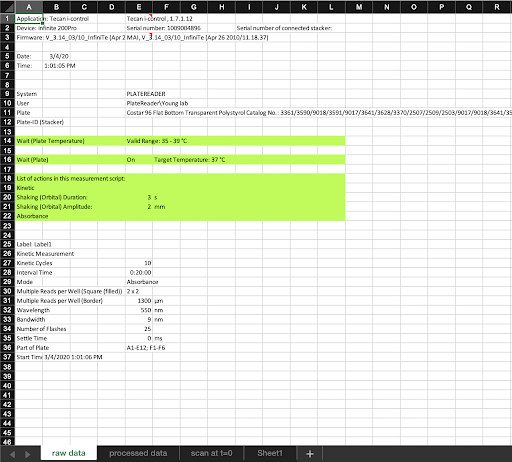
\includegraphics[width=.9\linewidth]{./docs/process_plate_reader_data_image01.png}
\end{center}
\begin{center}
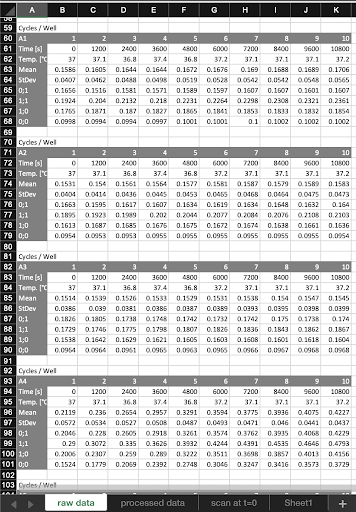
\includegraphics[width=.9\linewidth]{./docs/process_plate_reader_data_image02.png}
\end{center}
\begin{itemize}
\item NOTE: your file name must not have spaces! Rename it to have no spaces (just use underscores \_ ). This is good coding practice.

\item It is \textbf{imperative} that you do not edit the raw data. If you remove the any of the tables for wells that did not have samples, the script will fail. Version 2.0.0: I am working on a solution to this.
\end{itemize}

\item Your plate reader setup must be a .csv that looks like the example
below.

\begin{enumerate}
\item You MUST have the headers "row..1..2\ldots{}.12" AND the row letters in
CAPS!
\item Name all replicates EXACTLY the same (just copy and paste)
\begin{itemize}
\item \textbf{Version 2.0.0 Update}: Your sample names can be anything EXCEPT for "All".
\end{itemize}
\item \textbf{Label your media-only wells as Blank}
\item Leave empty wells blank
\begin{itemize}
\item \textbf{Version 2.0.0 Update}: If you have any wells that were scanned, but you do not want to include the data in the final output, just leave those wells blank in the plate setup file. The code will automatically ignore them.
\end{itemize}
\item Make sure there are not any extra spaces anywhere
\item You can make a .csv file in excel. Just save it as .csv
\begin{itemize}
\item Your sample names can now be whatever you want, as long as replicates are named \uline{EXACTLY} the same.
\item However, I would suggest you use actual sample names instead of a code.
\end{itemize}

\begin{center}
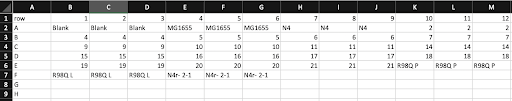
\includegraphics[width=.9\linewidth]{./docs/process_plate_reader_data_image03.png}
\end{center}
\end{enumerate}
\end{enumerate}

\section*{S3: USAGE}
\label{sec:org7bbbb03}
\begin{enumerate}
\item At the command line, once the script and your input files are in the
same directory, you can use this code like this:

\lstset{breaklines=true,language=bash,label= ,caption= ,captionpos=b,numbers=none}
\begin{lstlisting}
python process_plate_reader_data.py -i <rawdata.xlsx> -p <plate_setup.csv> -a <active_sheet_num>
\end{lstlisting}

\item A complete command could look like this:

\lstset{breaklines=true,language=bash,label= ,caption= ,captionpos=b,numbers=none}
\begin{lstlisting}
python process_plate_reader_data.py -i 200221_CCM_n4_lysis_curve_testing.xlsx -p 200221_plate_setup.csv -a 1
\end{lstlisting}

\item There are several arguments that can be input when you call the
script, but the 3 that are most important are -i, -p, and -a.

\item -i specifies the input data file
\item -p specifies the plate reader setup
\item -a specifies the sheet from your input data that has the raw data
\item \textbf{Note: computers count from 0}, so down below, I would enter 0
(actually you wouldn't have to do anything because the default setting
is the first sheet). If the second sheet had the data, I would enter
\begin{enumerate}
\item 
\end{enumerate}
\item Additionally, for help you can pass -h as your argument to get the
list of possible args

\begin{center}

\includegraphics[width=.9\linewidth]{./docs/process_plate_reader_data_image04.png}
\end{center}

Sheet = 0 Sheet = 1 Sheet = 2 Sheet = 3

\item Here are all the possible arguments you can pass and their
descriptions:
\end{enumerate}

\begin{center}
\begin{xltabular}{\textwidth}{lX}
Arg & Description\\
\hline
-i & input must be a .xlsx excel file from infinite200 pro plate reader tecan i-control 1.7.1.12 software\\
\hline
-p & plate setup file must be structured a certain way as a .csv -- see the example\\
 & NOTE: replicates must be named exactly the same AND your background media samples called "Blank"\\
 & Should you have samples you don't want analyzed or wells that were scanned but you don't want analyzed, label them as "air"\\
\hline
-a & type an integere for the sheet in your .xlsx file with the raw data\\
 & NOTE: computers start counting at 0 so if your 2nd sheet has the data, type "1"\\
 & DEFAULT=0 (first sheet)\\
\hline
-gs & type your intended graphing program\\
 & options: "excel", "R" DEFAULT="R"\\
 & "excel" will output wide formatted data\\
 & "R" will output long formatted data for use in R with ggplot2\\
\hline
-pp & bool to autogenerate a python plot\\
 & DEFAULT=True\\
 & Note: To set this to false, you need to pass \texttt{-pp} on the command line with nothing else. The script will automatically set this to False.\\
 & \textbf{Version 2.0.0} To produce a plot, the data must be long formatted, ie you must have the \texttt{-gs} parameter \texttt{R}.\\
\hline
-y & y-axis label\\
 & DEFAULT="OD600"\\
\hline
-gm & type of graphing method for python created graph\\
 & options: "time series", "time diff" DEFAULT="time series"\\
 & NOTE passing "time diff" does nothing yet TODO\\
\hline
-pw & type an integer for number of points (readings) per well\\
 & DEFAULT=4\\
 & \textbf{Version 2.0.0}: Deprecated. This is calculated from metadata in excel file.\\
\hline
-ts & \textbf{Version 2.0.0} Time scale. Determines what time scale is output in both the returned processed data and plots\\
 & Options: "sec", "min", "hr"\\
 & Default="hr".\\
\hline
-o & \textbf{Version 2.0.0} Output directory. Specify where you want the output files.\\
 & Default="output"\\
\hline
-fd & \textbf{Version 2.0.0} Figure dimensions. When the python plot is produced, specify the dimensions of the plot in \uline{inches}.\\
 & Default=(10,10)\\
 & Usage: To change this parameter, type \texttt{(w, h)} WITH the quotes.\\
\end{xltabular}
\end{center}

\section*{S4: HOW DOES IT WORK}
\label{sec:orgef78a56}

\begin{enumerate}
\item The code takes your plate setup file, and groups all replicates
together. Then it will find the well coordinates for all data in your
plate, grouping the coordinates for replicates together.

\item Then it parses all the data tables in your raw data file and matches
the data table with a sample labeled in your plate setup file.

\item Then it will concatenate all data tables together for all replicates
of a single experimental group. In other words, if you have 3
replicates of "rapid\_lyser\_2" in wells B2, B3, and B4, it will take
the data for wells B2, 3, and 4, and create one data table of all 3
replicates for "rapid\_lyser\_2."

\item Then it takes the average and standard deviation of all data points
for a given experimental group at each timepoint. For the tecan
i-control software, the data includes a certain number of readings
per well, and then that number is multiplied by the number of
replicates. The default readings per well number is 4, and if you
have 3 replicates, that equals 12 data points for each group at each
timepoint.

\item The average background signal at each timepoint is then subtractedOo
from the average signal at the corresponding timepoint for each
experimental group. This value is what is present in the final
output. Additionally, the unchanged standard deviation is also
reported in the final output because it will not change by
subtracting background signal. (See statistic distribution theory)

\item For the time series plotting, it will plot the relative time (hours)
on the x-axis, and whatever units your measurements are in on the
y-axis. For each point, it will also graph the standard error of the
mean OD \textpm{} SEM. at that timepoint. SEM = standard dev / sqrt(n), where
n is the number of replicates * number of readings per well.

\item The outputs of this code are a \texttt{datafile\_PROCESSED.csv} file and a
\texttt{datafile\_PROCESSED.pdf} file. The .csv file contains for all
experimental groups, the average signal (with background subtracted)
and standard deviation at each timepoint, as well as the time in
hours (by default). The .pdf is a python plot.
\end{enumerate}
\end{document}
